\chapter{模板使用简单说明}\label{chap:guide}

\section{文档目录简介}

\subsection{Thesis.tex}

Thesis.tex 为主文档,其设计和规划了论文的整体框架,通过对其的阅读可以了解整个论文框架的搭建。

\subsection{Style文件夹}

包含 nwsuafthesis 文档类的定义文件和配置文件,通过对它们的修改可以实现特定的模版设定。若需更新模板,一般只需用新的样式文件替换旧的即可。

\begin{enumerate}
    \item nwsuafthesis.cls:文档类定义文件,论文的最核心的格式即通过它来定义的。
    \item nwsuafthesis.cfg:文档类配置文件,设定如目录显示为“目~录”而非“目录”。
    \item artratex.sty: 常用宏包及文档设定,如参考文献样式、文献引用样式、页眉页脚设定等。这些功能具有开关选项,常只需在Thesis.tex中的如下命令中进行启用即可,一般无需修改artratex.sty本身。
        
        \path{\usepackage[options]{artratex}} 
    \item artracom.sty:自定义命令以及添加宏包的推荐放置位置。
\end{enumerate}

\subsection{Tex文件夹}

文件夹内为论文的所有实体内容,详细分类介绍如下:

\begin{itemize}
    \item 01\_Frontpage.tex:为论文中英文封面及中英文摘要。
    \item 03\_Mainmatter.tex:索引需要出现的Chapter。开始写论文时,可以只索引当前章节,以快速编译查看,当论文完成后,再对所有章节进行索引即可。
    \item 03x\_Chap\_xxx.tex:为论文主体的各个章节,可根据需要添加和撰写。
    \item 04\_Appendix.tex:为附录内容
    \item 05\_Backmatter.tex:为发表文章信息和致谢部分等。
\end{itemize}

\subsection{Img文件夹}

用于放置论文中所需要的图类文件,支持格式有:.jpg, .png, .pdf。其中,\verb|nwsuaf_logo.pdf|为西农大校徽。不建议为各章节图片建子目录,即使图片众多,若命名规则合理,图片查询亦是十分方便。

\subsection{Biblio文件夹}

\begin{enumerate}
    \item ref.bib:参考文献信息库。
    \item gbt7714-xxx.bst:符合国标的文献样式定义文件。由 \href{https://github.com/zepinglee/gbt7714-bibtex-style}{zepinglee}  开发,并满足最新国标要求。与文献样式有关的问题,请查阅开发者所提供的文档,并建议适当追踪其更新。
\end{enumerate}

\section{数学公式、图表、参考文献等功能}

\subsection{数学公式}

比如Navier-Stokes方程:
\begin{equation} \label{eq:ns}
    \begin{cases}
        \frac{\partial \rho}{\partial t} + \nabla\cdot(\rho\Vector{V}) = 0 \ \mathrm{times\ font\ test}\\
        \frac{\partial (\rho\Vector{V})}{\partial t} + \nabla\cdot(\rho\Vector{V}\Vector{V}) = \nabla\cdot\Tensor{\sigma} \ \text{times font test}\\
        \frac{\partial (\rho E)}{\partial t} + \nabla\cdot(\rho E\Vector{V}) = \nabla\cdot(k\nabla T) + \nabla\cdot(\Tensor{\sigma}\cdot\Vector{V})
    \end{cases}
\end{equation}
\begin{equation}
    \frac{\partial }{\partial t}\int\limits_{\Omega} u \, \mathrm{d}\Omega + \int\limits_{S} \unitVector{n}\cdot(u\Vector{V}) \, \mathrm{d}S = \dot{\phi}
\end{equation}

数学公式常用命令请见 \href{https://en.wikibooks.org/wiki/LaTeX/Mathematics}{WiKibook Mathematics}。artracom.sty中对一些常用数据类型如矢量矩阵等进行了封装,这样的好处是如有一天需要修改矢量的显示形式,只需单独修改artracom.sty中的矢量定义即可实现全文档的修改。

\subsection{表格}

请见表~\ref{tab:sample}。制表的更多范例,请见 \href{https://en.wikibooks.org/wiki/LaTeX/Tables}{WiKibook Tables}。
\begin{table}[!htbp]
    \bicaption{这是一个样表。}{This is a sample table.}
    \label{tab:sample}
    \centering
    \footnotesize% fontsize
    \setlength{\tabcolsep}{4pt}% column separation
    \renewcommand{\arraystretch}{1.2}%row space 
    \begin{tabular}{lcccccccc}
        \hline
        Row number & \multicolumn{8}{c}{This is a multicolumn} \\
        %\cline{2-9}% partial hline from column i to column j
        \hline
        Row 1 & $1$ & $2$ & $4$ & $5$ & $6$ & $7$ & $8$\\
        Row 2 & $1$ & $2$ & $4$ & $5$ & $6$ & $7$ & $8$\\
        Row 3 & $1$ & $2$ & $4$ & $5$ & $6$ & $7$ & $8$\\
        Row 4 & $1$ & $2$ & $4$ & $5$ & $6$ & $7$ & $8$\\
        \hline
    \end{tabular}
\end{table}

\subsection{图片插入}

论文中图片的插入通常分为单图和多图,下面分别加以介绍:

单图插入:假设插入名为\verb|tc_q_criteria|(后缀可以为.jpg、.png、.pdf,下同)的图片,其效果如图\ref{fig:tc_q_criteria}。
\begin{figure}[!htbp]
    \centering
    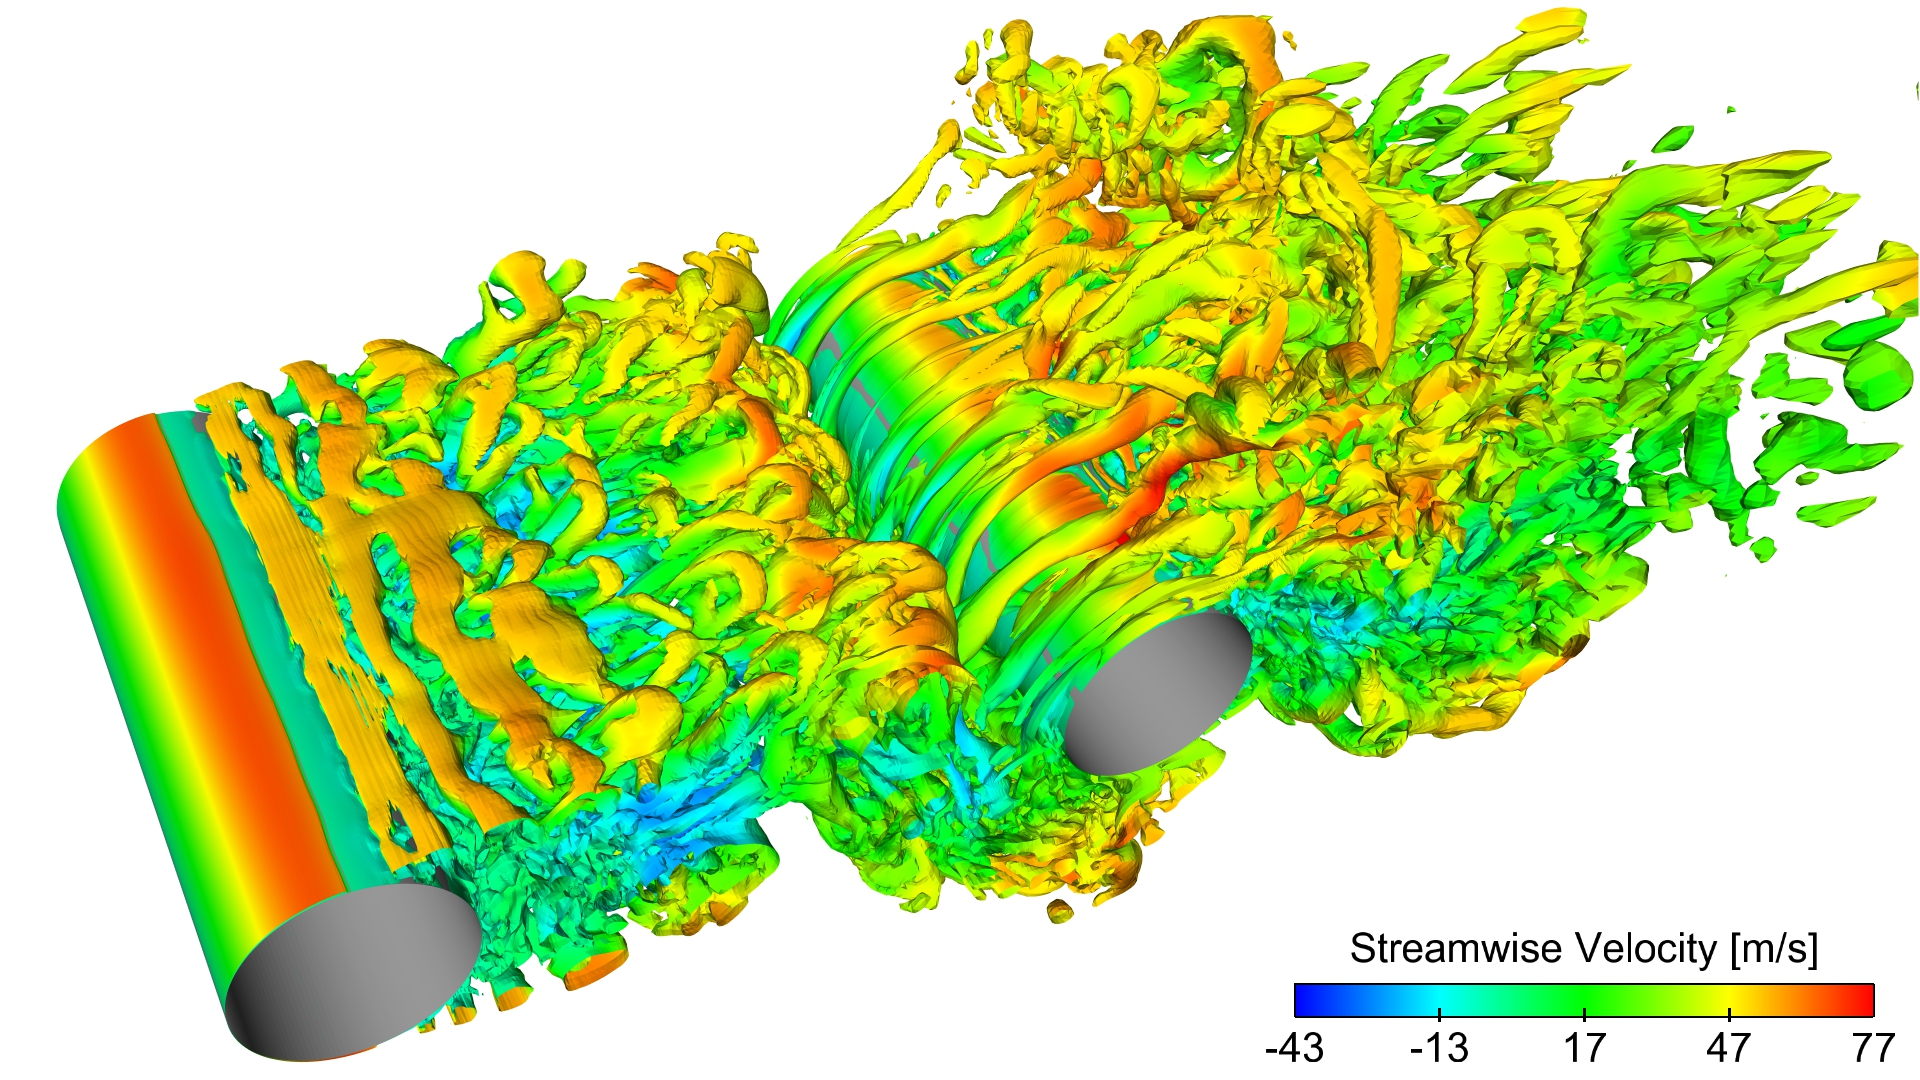
\includegraphics[width=0.40\textwidth]{tc_q_criteria}
    \bicaption{Q判据等值面图,同时测试一下一个很长的标题,比如这真的是一个很长很长很长很长很长很长很长很长的标题。}{Isocontour of Q criteria, at the same time, this is to test a long title, for instance, this is a really very long very long very long very long very long title.}
    \label{fig:tc_q_criteria}
\end{figure}

如果插图的空白区域过大,以图片\verb|shock_cyn|为例,自动裁剪如图\ref{fig:shock_cyn}。
\begin{figure}[!htbp]
    \centering
    %trim option's parameter order: left bottom right top
    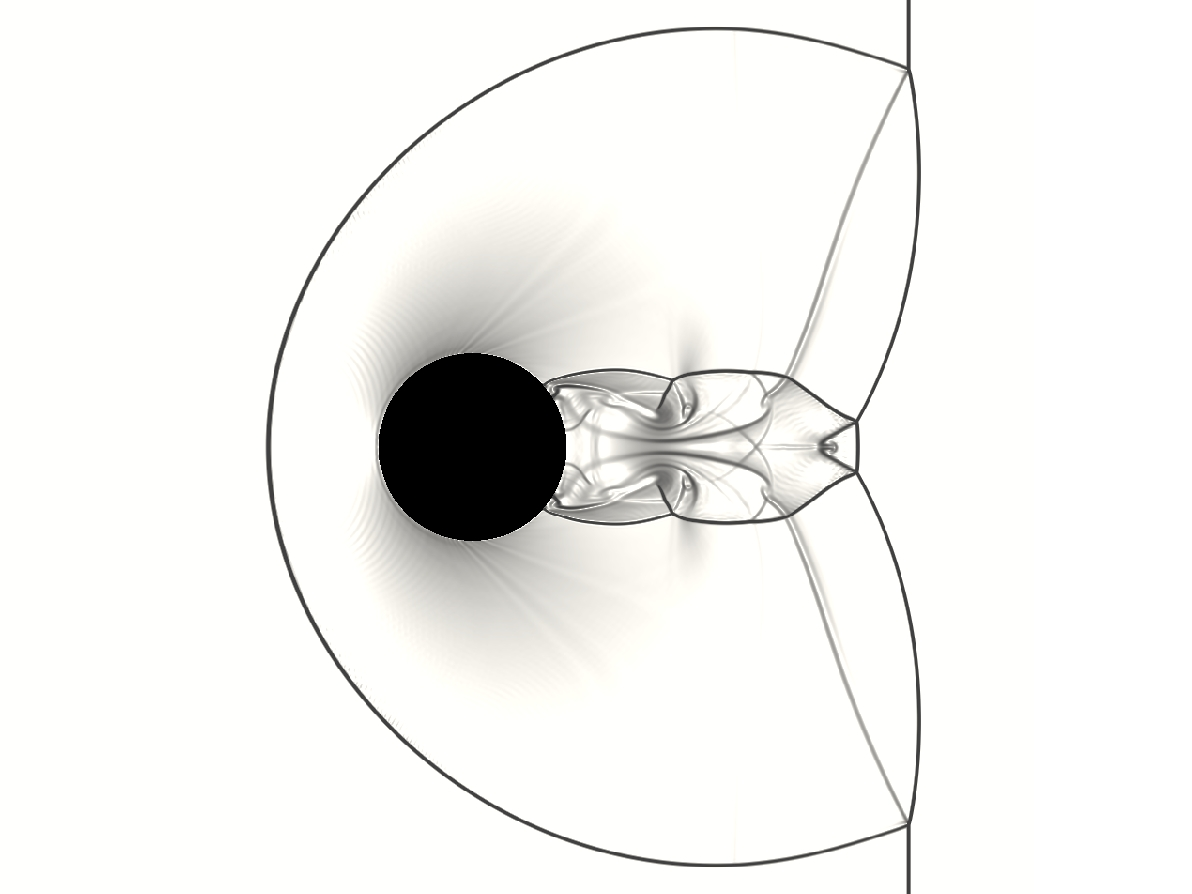
\includegraphics[trim = 30mm 0mm 30mm 0mm, clip, width=0.40\textwidth]{shock_cyn}
    \bicaption{激波圆柱作用。}{Shock-cylinder interaction.}
    \label{fig:shock_cyn}
\end{figure}

多图的插入如图\ref{fig:oaspl},多图不应在子图中给文本子标题,只要给序号,并在主标题中进行引用说明。
\begin{figure}[!htbp]
    \centering
    \begin{subfigure}[b]{0.35\textwidth}
      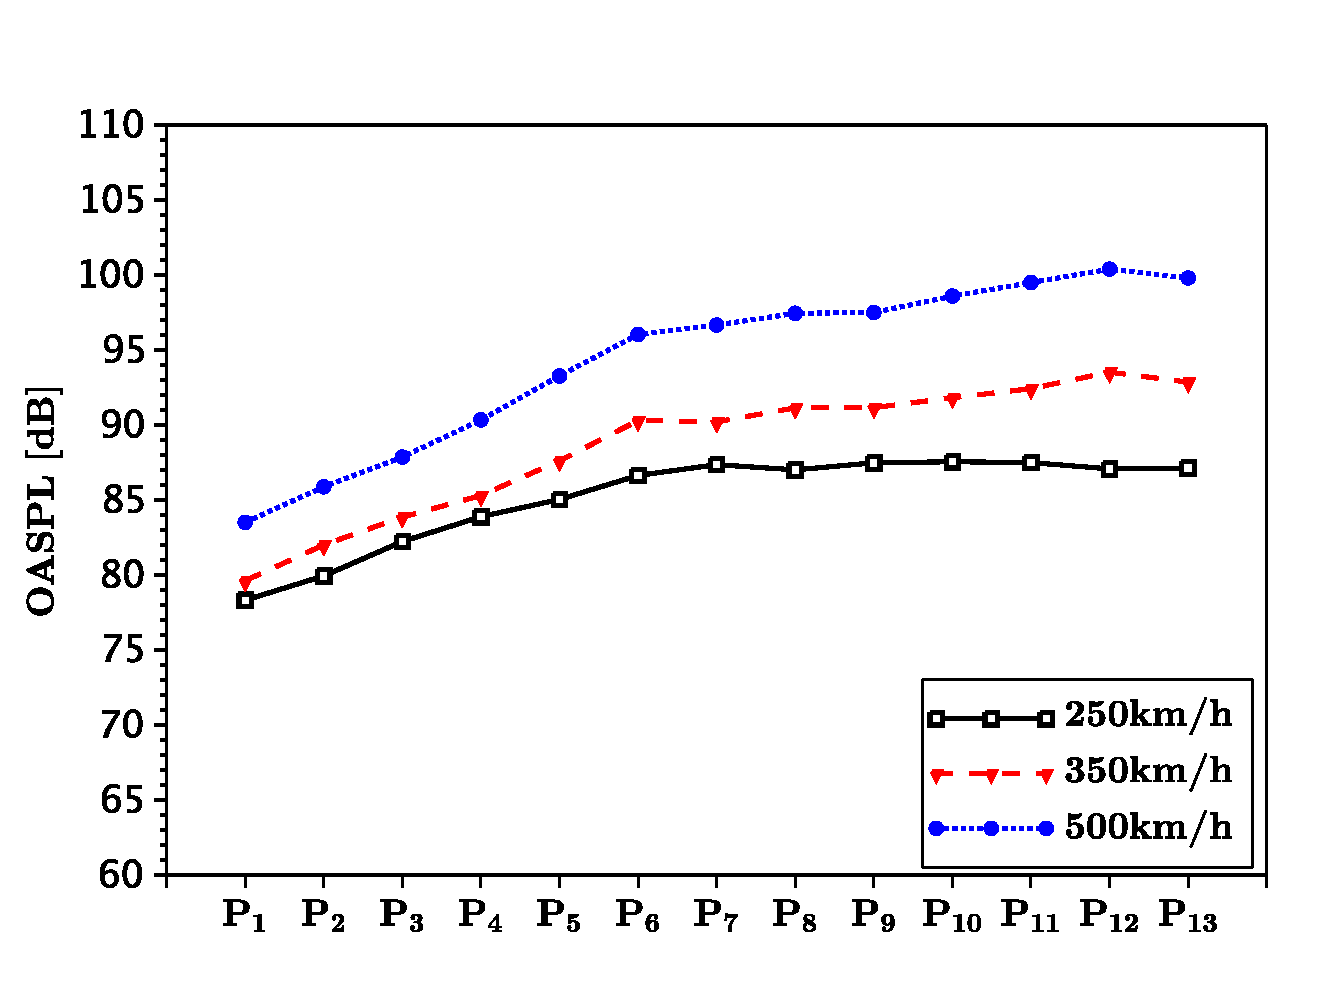
\includegraphics[width=\textwidth]{oaspl_a}
      \caption{}
      \label{fig:oaspl_a}
    \end{subfigure}%
    ~%add desired spacing
    \begin{subfigure}[b]{0.35\textwidth}
      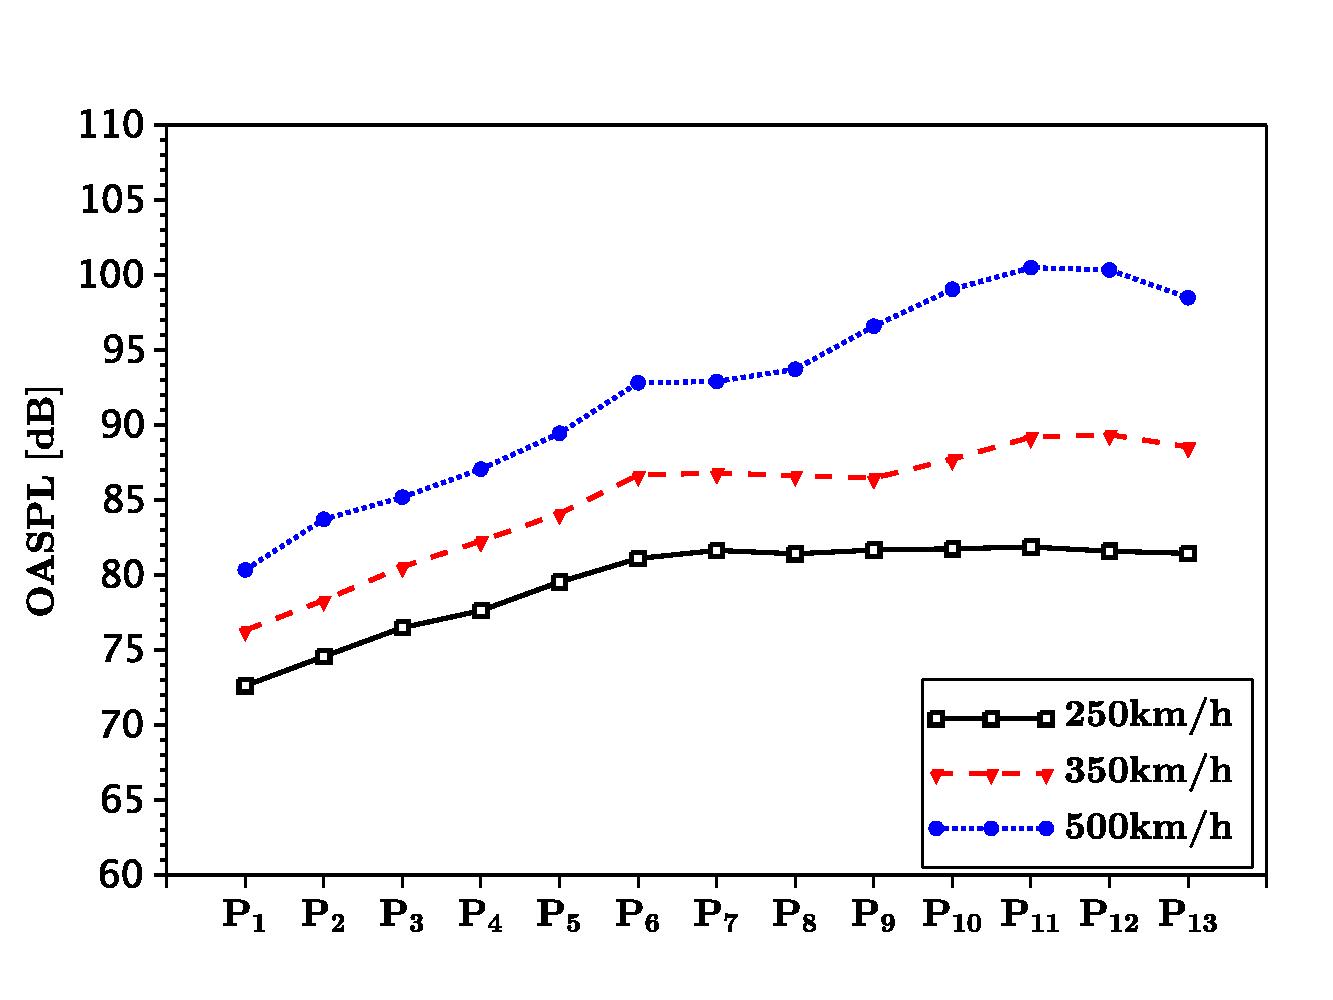
\includegraphics[width=\textwidth]{oaspl_b}
      \caption{}
      \label{fig:oaspl_b}
    \end{subfigure}
    \begin{subfigure}[b]{0.35\textwidth}
      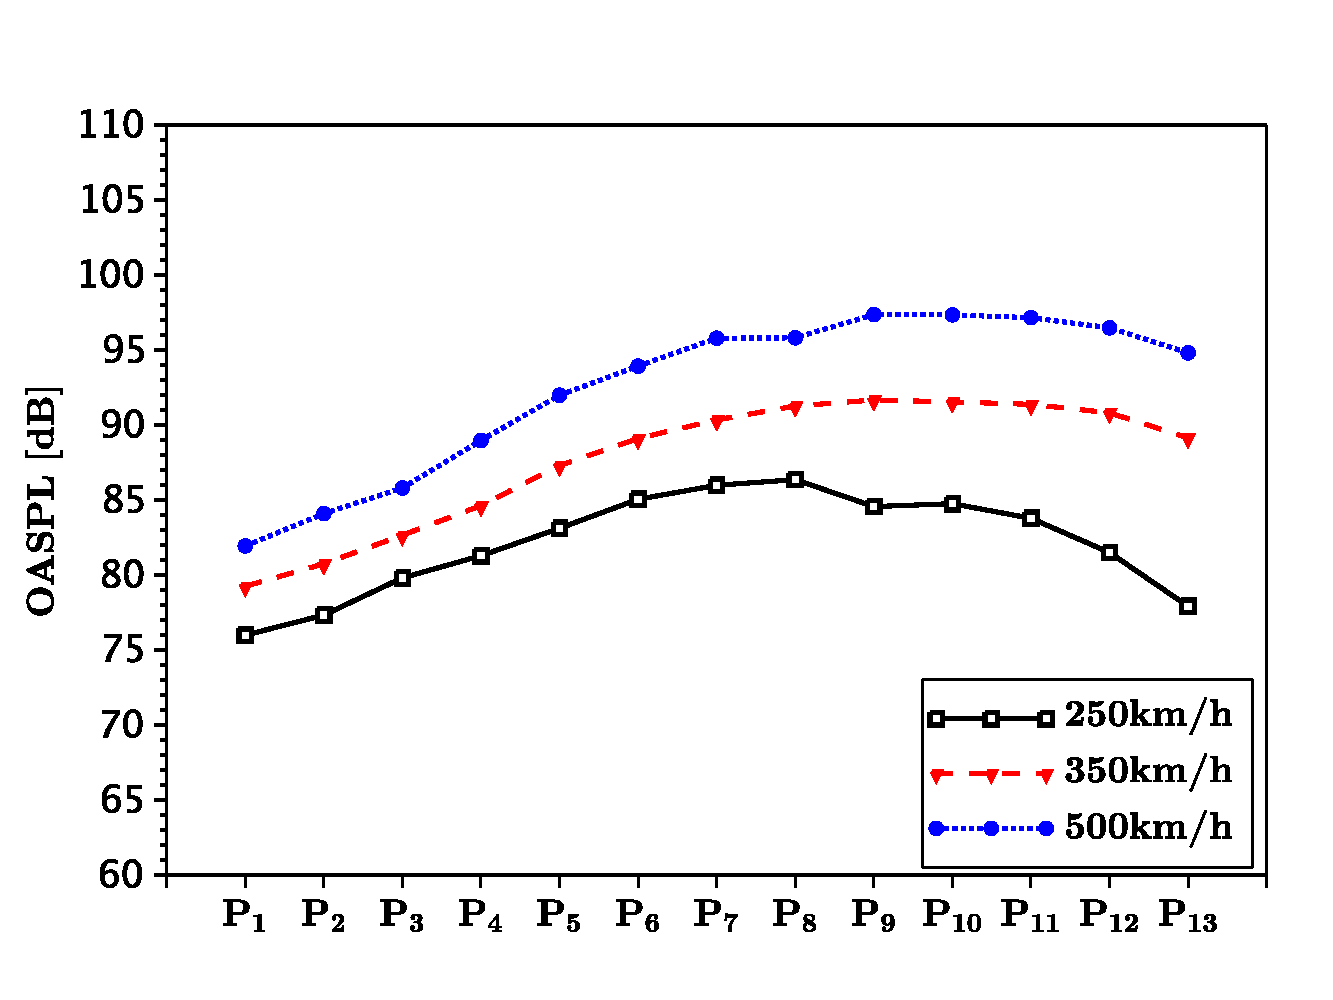
\includegraphics[width=\textwidth]{oaspl_c}
      \caption{}
      \label{fig:oaspl_c}
    \end{subfigure}%
    ~%add desired spacing
    \begin{subfigure}[b]{0.35\textwidth}
      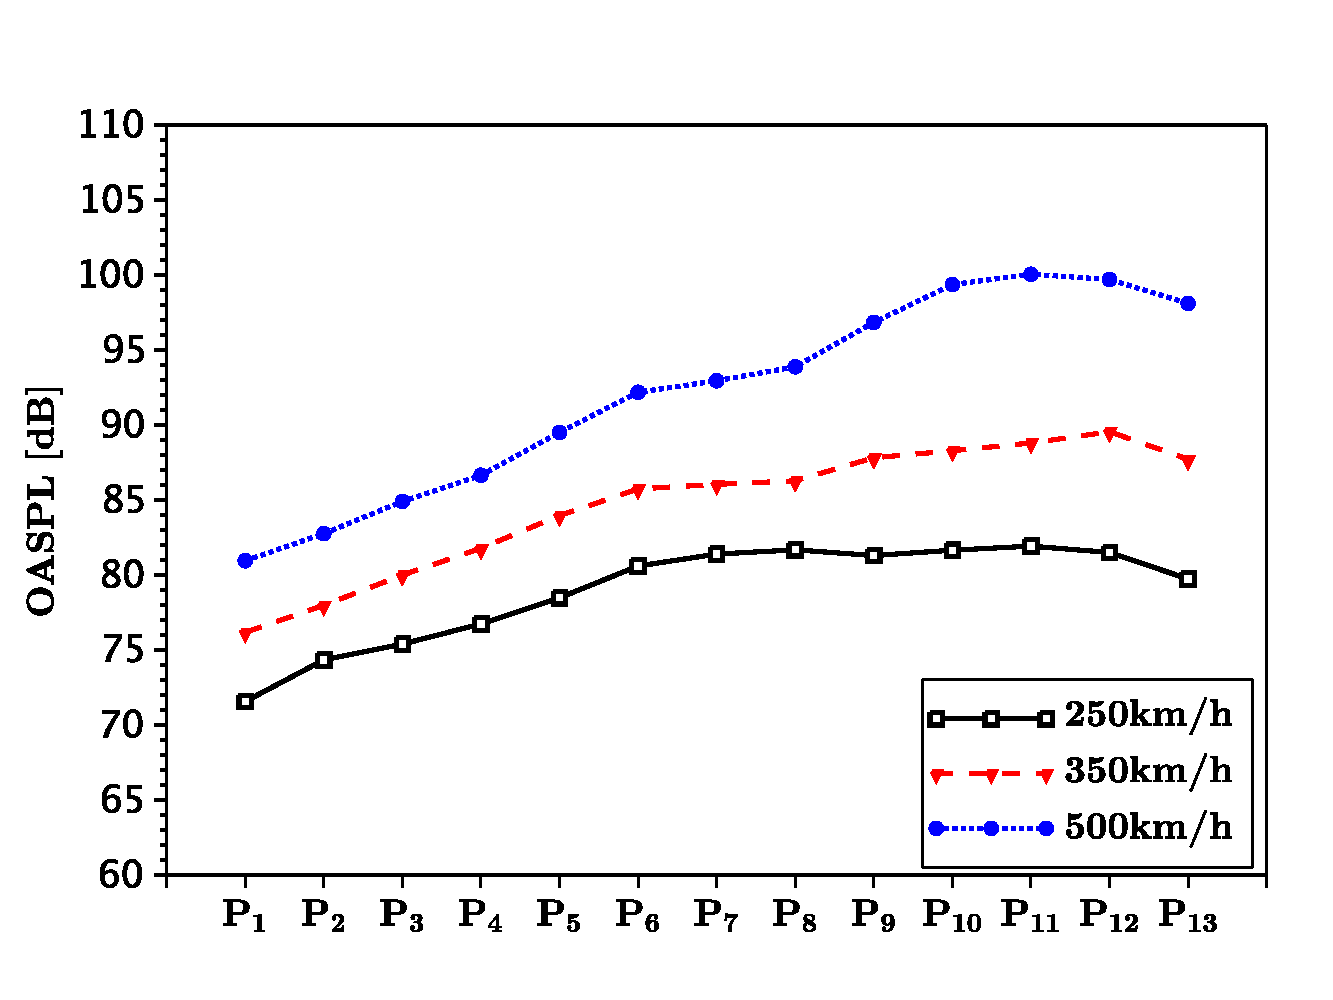
\includegraphics[width=\textwidth]{oaspl_d}
      \caption{}
      \label{fig:oaspl_d}
    \end{subfigure}
    \bicaption{总声压级。(a) 这是子图说明信息,(b) 这是子图说明信息,(c) 这是子图说明信息,(d) 这是子图说明信息。}{OASPL.(a) This is the explanation of subfig, (b) This is the explanation of subfig, (c) This is the explanation of subfig, (d) This is the explanation of subfig.}
    \label{fig:oaspl}
\end{figure}

\subsection{算法}

如见算法~\ref{alg:euclid},详细使用方法请参见文档 \href{https://ctan.org/pkg/algorithmicx?lang=en}{algorithmicx}。

\begin{algorithm}[!htbp]
    \small
    \caption{Euclid's algorithm}\label{alg:euclid}
    \begin{algorithmic}[1]
        \Procedure{Euclid}{$a,b$}\Comment{The g.c.d. of a and b}
        \State $r\gets a\bmod b$
        \While{$r\not=0$}\Comment{We have the answer if r is 0}
        \State $a\gets b$
        \State $b\gets r$
        \State $r\gets a\bmod b$
        \EndWhile\label{euclidendwhile}
        \State \textbf{return} $b$\Comment{The gcd is b}
        \EndProcedure
    \end{algorithmic}
\end{algorithm}

\subsection{参考文献引用}

参考文献引用过程以实例进行介绍,假设需要引用名为"Document Preparation System"的文献,步骤如下:

1)使用Google Scholar搜索Document Preparation System,在目标条目下点击Cite,展开后选择Import into BibTeX打开此文章的BibTeX索引信息,将它们copy添加到ref.bib文件中(此文件位于Biblio文件夹下)。

2)索引第一行 \verb|@article{lamport1986document,|中 \verb|lamport1986document| 即为此文献的label (\textbf{中文文献也必须使用英文label},一般遵照:姓氏拼音+年份+标题第一字拼音的格式),想要在论文中索引此文献,有两种索引类型:

文本类型:\verb|\citet{lamport1986document}|。正如此处所示 \citet{lamport1986document}; 

括号类型:\verb|\citep{lamport1986document}|。正如此处所示 \citep{lamport1986document}。

\textbf{多文献索引用英文逗号隔开}:

\verb|\citep{lamport1986document, chu2004tushu, chen2005zhulu}|。正如此处所示 \citep{lamport1986document, chu2004tushu, chen2005zhulu}

更多例子如:

\citet{walls2013drought}根据...的研究,首次提出...。其中关于...\citep{walls2013drought},是当前中国...得到迅速发展的研究领域\citep{chen1980zhongguo}。引用同一著者在同一年份出版的多篇文献时,在出版年份之后用
英文小写字母区别,如:\citep{yuan2012lana, yuan2012lanb, yuan2012lanc}。同一处引用多篇文献时,按出版年份由近及远依次标注,中间用
分号分开。例如\citep{chen1980zhongguo, stamerjohanns2009mathml, hls2012jinji, niu2013zonghe}。

使用著者-出版年制(authoryear)式参考文献样式时,中文文献必须在BibTeX索引信息的 \textbf{key} 域(请参考ref.bib文件)填写作者姓名的拼音,才能使得文献列表按照拼音排序。参考文献表中的条目(不排序号),先按语种分类排列,语种顺 序是:中文、日文、英文、俄文、其他文种。然后,中文按汉语拼音字母顺序排列,日文按第一著者的姓氏笔画排序,西文和 俄文按第一著者姓氏首字母顺序排列。如中\citep{niu2013zonghe}、日\citep{Bohan1928}、英\citep{stamerjohanns2009mathml}、俄\citep{Dubrovin1906}。

如此,即完成了文献的索引,请查看下本文档的参考文献一章,看看是不是就是这么简单呢?是的,就是这么简单!

不同文献样式和引用样式,如著者-出版年制(authoryear)、顺序编码制(numbers)、上标顺序编码制(super)可在Thesis.tex中对artratex.sty调用实现,如:
\begin{itemize}
    \footnotesize
    \item \verb+\usepackage[numbers]{artratex}+ $\%$ 文本: Jones [1]; 括号: [1]
    \item \verb+\usepackage[super]{artratex}+ $\%$ 文本: Jones 上标[1]; 括号: 上标[1]
    \item \verb+\usepackage[authoryear]{artratex}+ $\%$ 文本: Jones (1995); 括号: (Jones, 1995)
    \item \verb+\usepackage[alpha]{artratex}+ $\%$ 文本: 不可用; 括号: [Jon95]
\end{itemize}

当前文档的默认参考文献样式为\textbf{authoryear}。若在上标(\textbf{super})模式下,希望在特定位置将上标改为嵌入式标,可使用

文本类型:\verb|\citetns{lamport1986document,chen2005zhulu}|。

正如此处所示\citetns{lamport1986document,chen2005zhulu}

括号类型:\verb|\citepns{lamport1986document,chen2005zhulu}|。

正如此处所示\citepns{lamport1986document,chen2005zhulu}

参考文献索引更为详细的信息,请见 \href{https://github.com/zepinglee/gbt7714-bibtex-style}{zepinglee} 和 \href{https://en.wikibooks.org/wiki/LaTeX/Bibliography_Management}{WiKibook Bibliography}。

\nocite{*}


\section{字体切换}

\begin{itemize}
    \item 宋体:西农大论文模板nwsuafthesis 或 \textrm{西农大论文模板nwsuafthesis}
    \item 粗宋体:{\bfseries 西农大论文模板nwsuafthesis} 或 \textbf{西农大论文模板nwsuafthesis}
    \item 黑体:{\sffamily 西农大论文模板nwsuafthesis} 或 \textsf{西农大论文模板nwsuafthesis}
    \item 粗黑体:{\bfseries\sffamily 西农大论文模板nwsuafthesis} 或 \textsf{\bfseries 西农大论文模板nwsuafthesis}
    \item 仿宋:{\ttfamily 西农大论文模板nwsuafthesis} 或 \texttt{西农大论文模板nwsuafthesis}
    \item 粗仿宋:{\bfseries\ttfamily 西农大论文模板nwsuafthesis} 或 \texttt{\bfseries 西农大论文模板nwsuafthesis}
    \item 楷体:{\itshape 西农大论文模板nwsuafthesis} 或 \textit{西农大论文模板nwsuafthesis}
    \item 粗楷体:{\bfseries\itshape 西农大论文模板nwsuafthesis} 或 \textit{\bfseries 西农大论文模板nwsuafthesis}
\end{itemize}





